%%%%%%%%%%%%%%%%%%%%%%%%%%%%%%%%%%%%%%%%%%%%%%%%%%%%%%%%%%%%%%%%%%%%%%%%%%%%%%%%%
% MICAI / Springer LNCS submission -- COMPACT (deliverable) version, 2026-06-12
% Restructured from the frozen 20pp main_reducida.tex toward MICAI-2025 norms
% (~16-17pp): methodology pipeline diagram, Pareto+FIFO figure, annotated 2x2
% mechanism figure (absorbs the factorial table), cross-structure rank figure
% (replaces the rank table), operators table -> prose, Taguchi section inlined.
% Every retained number is verbatim from the frozen version (firewall-covered).
% FROZEN BASES (do not edit): main.tex, main_submission.tex, main_reducida.tex,
% main_reducida_submission.tex.
%
% Compile: pdflatex main_compacta  (x2-3 passes to resolve refs)
% Bibliography: inline thebibliography (no BibTeX pass needed).
%
% ---------------------------------------------------------------------------
% DOUBLE-BLIND SUBMISSION:  MICAI reviews anonymously. To anonymize, (1) comment
% out the \author / \institute blocks below and use the ANONYMOUS block marked
% "% >>> REVIEW", (2) comment out the Acknowledgements, and (3) remove the repo
% URL in the Data Availability statement. The body is otherwise identical.
%%%%%%%%%%%%%%%%%%%%%%%%%%%%%%%%%%%%%%%%%%%%%%%%%%%%%%%%%%%%%%%%%%%%%%%%%%%%%%%%%
\documentclass[runningheads]{llncs}

% --- A4 trap fix: force a true A4 MediaBox without touching the LNCS text block.
\AtBeginDocument{\pdfpagewidth=210mm \pdfpageheight=297mm}

\usepackage[T1]{fontenc}
\usepackage[utf8]{inputenc}
\usepackage{lmodern}   % scalable fonts (required for microtype expansion)
\usepackage{graphicx}
\usepackage{xcolor}
% amsmath + llncs emit one benign "Unable to redefine math accent \vec" warning
% (modern robust accents); silence just that during amsmath's load, then restore.
\makeatletter
\let\vp@oldwarn\PackageWarningNoLine
\renewcommand\PackageWarningNoLine[2]{}
\usepackage{amsmath,amssymb}
\let\PackageWarningNoLine\vp@oldwarn
\makeatother
\setlength{\emergencystretch}{1em}  % gentle: absorb tight lines in narrow columns
\usepackage{booktabs}
\usepackage{array}
\usepackage{tikz}
\usetikzlibrary{arrows.meta,positioning,fit,backgrounds}
\usepackage{microtype}
\usepackage[hidelinks]{hyperref}
\usepackage{url}
\renewcommand\UrlFont{\color{black}\rmfamily}

% consistent metric/acronym capitalization
\newcommand{\HV}{\textsf{HV}}
\newcommand{\IGD}{\textsf{IGD}}

\graphicspath{{figures/}}

\begin{document}

\title{A Two-Condition Diagnostic for Decoder-Based\texorpdfstring{\\}{ }Multi-Objective Search: When Blind Sampling\texorpdfstring{\\}{ }Beats a Mismatched NSGA-II}
\titlerunning{Two-Condition Diagnostic for Decoder-Based Search}

% >>> CAMERA-READY (named) author block:
\author{Javier Augusto Rebull Saucedo\orcidID{0009-0008-2089-5274} \and
Yazmin Ivonne Flores Martinez\orcidID{0009-0002-6848-1608} \and
Ra\'ul Gibran Porras Alaniz\orcidID{0000-0002-6772-5351}}
\authorrunning{J.\,A. Rebull Saucedo et al.}
\institute{Maestr\'ia en Inteligencia Artificial y Anal\'itica de Datos, Universidad Aut\'onoma de Ciudad Ju\'arez, Ciudad Ju\'arez, Chihuahua, M\'exico\\
\email{rebull@outlook.com}}

% >>> REVIEW (anonymous) author block -- swap in for double-blind submission:
% \author{Anonymous Author(s)}
% \authorrunning{Anonymous}
% \institute{Institution withheld for review}

\maketitle

\begin{abstract}
Many hard-constrained combinatorial problems are solved by pairing a metaheuristic with a feasibility-preserving decoder, yet the true driver of performance is seldom isolated. We isolate it on a calibrated case study: allocating 140{,}000 U.S.\ employment-based visas per year under a per-country ceiling and spillover cascade---a three-objective integer program with six hard constraints, searched through a random-key decoder whose allocations are feasible by construction---no penalties, no repair. A controlled nine-method ladder shows why search fails. Blind random sampling beats a standard real-coded NSGA-II and a naive swarm because their realized search is \emph{degenerate}: interpolating operators barely change the decoded order, or gated acceptance freezes the population. The two corresponding conditions are necessary there, not sufficient: a BRKGA-style order-changing crossover only ties blind sampling, and a registered disruption sweep finds hypervolume nearly flat within that family---only the right kind of order renewal reaches the top tier. We package these measurements as a cheap a priori screening diagnostic and stress it with registered prospective tests: the two-condition core predicted correctly; the landscape label did not. Across knapsack, traveling-salesman, flow-shop, and set-covering replications, the best ladder method satisfies both conditions, while the mismatched genetic algorithm's collapse below blind sampling is landscape- and configuration-specific. A Taguchi design fixes the shared parameters; the recovered front Pareto-dominates the first-in, first-out incumbent.

\keywords{Multi-objective optimization \and Harris Hawks Optimization \and Constraint handling \and Random-key decoder \and Permutation encoding \and Taguchi design of experiments \and Resource allocation}
\end{abstract}

%===============================================================================
\section{Introduction}
\label{sec:intro}

Each fiscal year the United States Congress authorizes approximately 140{,}000 employment-based (EB) immigrant visas, distributed across five categories (EB-1 to EB-5). Two structural rules govern the distribution: a \emph{per-country ceiling} ($P_c \approx 25{,}620$ visas, the statutory 7\,\% cross-preference limit~\cite{uscis}) that no single country may exceed, and a \emph{spillover} mechanism that cascades unused visas across categories (EB-4/5 $\rightarrow$ EB-1 $\rightarrow$ EB-2 $\rightarrow$ EB-3). The incumbent system processes petitions strictly first-in, first-out (FIFO) by priority date. In our calibrated instance these rules create measurable inefficiencies: two countries hold roughly three-quarters of demand (India $\approx 63\,\%$, China $\approx 14\,\%$) with 10--13-year waits, while the ceiling clash leaves thousands of visas unused.

This matters beyond accounting: behind every backlogged petition is a household whose relocation and reunification hinge on a priority date. The problem admits three legitimate, mutually conflicting goals: serve the longest-waiting petitions (\emph{efficiency}), distribute opportunity evenly across nationalities (\emph{equity}), and waste no visas (\emph{utilization}). No single allocation optimizes all three; the decision-relevant object is the set of best compromises---a Pareto front. Algorithmic assignment of people to scarce slots has been studied for refugee resettlement~\cite{bansak}; our contribution is methodological, not a new matching design.

Computing that front is hard: the allocation is \emph{combinatorial} (integer visa counts for 105 country$\times$category groups under six simultaneous constraints, a feasible set generalizing the NP-hard multidimensional knapsack~\cite{garey}), the objectives genuinely conflict, and the \emph{hard constraints} are unforgiving---a continuous metaheuristic naturally proposes infeasible candidates, and aggressive repair or penalties either require delicate tuning or distort the search landscape.

We address these challenges with a multi-objective adaptation of Harris Hawks Optimization (MOHHO) whose centerpiece is a \emph{feasibility-preserving decoder}. Our central contribution is methodological: a controlled, mechanistically explained account of when decoder-based search beats blind sampling, distilled into a two-condition diagnostic that a practitioner can run before committing a full experimental budget. Concretely, this paper contributes \emph{(i)}~a decoder that couples a smallest-position-value (SPV) random-key mapping with a deterministic greedy assignment, guaranteeing all six hard constraints \emph{by construction}; \emph{(ii)}~a calibrated, constraint-heavy case study on which a multi-objective Harris Hawks optimizer recovers a Pareto front of policy trade-offs that dominates the FIFO incumbent; \emph{(iii)}~a Taguchi L9 design that fixes the parameters shared by every ladder method, so that cross-method comparisons are not confounded by per-method tuning; \emph{(iv)}~a controlled nine-method ladder, a $2\times2$ isolation experiment, and a direct operator-order-preservation measurement (Kendall $\tau$ through the decoder), together yielding the two-condition diagnostic---operators must change the decoded order and selection must preserve diversity---sharpened by a predictive test from a binary conjunction to a necessary-but-graded rule; and \emph{(v)}~a reproducible protocol (30 seeds, omnibus Friedman tests with Nemenyi post-hocs and effect sizes, five perturbed-demand instances) and a four-structure generalization plus a registered prospective test on a fifth structure (set covering), separating what transfers from what is landscape- and configuration-specific (the collapse of a genetic algorithm (GA) below random sampling).

%===============================================================================
\section{Background and Related Work}
\label{sec:related}

Harris Hawks Optimization (HHO)~\cite{heidari}, a population-based metaheuristic driven by a prey \emph{escape energy} (Section~\ref{sec:mohho}), has been extended to multiple objectives via external archives, elitist non-dominated sorting, and grid indices~\cite{choo,jangir,cerci,kusoglu}; these variants are validated mostly on continuous benchmarks, leaving their use on constrained combinatorial allocation---where feasibility, not convergence, is the binding difficulty---comparatively unexplored.

We bridge continuous search and combinatorial structure with random keys~\cite{bean}: a real vector is decoded to a feasible permutation by sorting (the SPV rule~\cite{tasgetiren}). How much an operator step changes the decoded phenotype is the classical representation-\emph{locality} question, formalized by Rothlauf~\cite{rothlauf} and measured for decoder-based evolutionary algorithms by Raidl and Gottlieb~\cite{raidl}---the lens our Kendall-$\tau$ measurement instantiates (their \emph{heuristic-bias} half makes blind sampling through a greedy decoder a semi-greedy multistart in the GRASP (greedy randomized adaptive search procedure) sense~\cite{feo}). The idea underlies biased random-key genetic algorithms (BRKGA)~\cite{goncalves,londe}---whose uniform crossover exists precisely because interpolating operators move keys without moving the decoded order---and a general random-key optimizer pairing a decoder with any metaheuristic~\cite{chaves}, the paradigm we probe by varying the metaheuristic while holding the decoder fixed. Among constraint-handling families~\cite{rahimi}, penalty methods need problem-specific weights, repair can collapse diversity, and decoder (feasibility-preserving) approaches guarantee feasibility by construction; we adopt the third. NSGA-II (Non-dominated Sorting Genetic Algorithm~II)~\cite{deb} is our benchmark and the standard tool for hard allocation and scheduling~\cite{zhang}; our finding that the choice of metaheuristic family is second-order once operators match the representation speaks to the metaphor-centered critique of metaheuristics~\cite{aranha,sorensen}. We tune parameters with a Taguchi orthogonal array~\cite{alrafei,montgomery} and assess fronts with the hypervolume~\cite{zitzler}, inverted generational distance and spacing~\cite{coello}, nonparametric tests~\cite{derrac}, and the $A_{12}$ effect size~\cite{vargha}.

%===============================================================================
\section{Problem Formulation}
\label{sec:formulation}

\paragraph{Decision variables.}
The problem is discretized into $G = C \times |\mathcal{J}| = 21 \times 5 = 105$ \emph{groups}, where each group $g$ is a (country~$c$, category~$j$) pair. The decision vector is
\(
\mathbf{x} = (x_1, x_2, \dots, x_G),\; x_g \in \mathbb{Z}^{+}_0,
\)
where $x_g$ is the number of visas assigned to group $g$. Each group has a demand (backlog) $n_g$ and a \emph{waiting weight} $w_g = t_{\text{now}} - d_g$, the years elapsed since its priority date $d_g$.

\paragraph{Objectives.}
We minimize three conflicting objectives:
\begin{align}
f_1(\mathbf{x}) &= \frac{\sum_{g}(n_g - x_g)\,w_g}{\sum_{g} n_g}
&&\text{unserved waiting load (efficiency),}\\
f_2(\mathbf{x}) &= \max_{c_1,c_2 \in \mathcal{C}}\bigl|\bar{W}_{c_1} - \bar{W}_{c_2}\bigr|
&&\text{maximum inter-country disparity (equity),}\\
f_3(\mathbf{x}) &= V - \textstyle\sum_{g} x_g
&&\text{wasted (unassigned) visas (utilization),}
\end{align}
where $V$ is the total visa supply and $\bar{W}_c = \big(\sum_{g:\,c(g)=c} x_g w_g\big)\big/\big(\sum_{g:\,c(g)=c} x_g\big)$ is the visa-weighted mean wait of country $c$, so $f_2$ is the gap between the longest- and shortest-waiting nationalities. (An unserved country takes its worst backlog wait as $\bar{W}_c$---an anti-starvation convention; reported solutions serve every country.)

\paragraph{Constraints.}
The feasible set $\mathcal{F}$ is defined by six hard constraints:
\begin{align}
&\text{R1:}\; \textstyle\sum_{g} x_g \le V \text{ (total)}
&&\text{R2:}\; \textstyle\sum_{g:\,c(g)=c} x_g \le P_c \;\forall c \text{ (country)}\nonumber\\
&\text{R3:}\; \textstyle\sum_{g:\,j(g)=j} x_g \le K_j^{\text{eff}} \;\forall j \text{ (category)}
&&\text{R4:}\; 0 \le x_g \le n_g \;\forall g \text{ (demand)}\nonumber\\
&\text{R5:}\; x_g \in \mathbb{Z}^{+}_0 \;\forall g \text{ (integrality)}
&&\text{R6:}\; \text{FIFO order within each } (c,j) \text{ queue}\nonumber
\end{align}
where $K_j^{\text{eff}}$ is the per-category cap after the spillover cascade. We use the statutory ceiling as an exogenous annual EB-side cap in this single-year model (a full legal simulation of family-sponsored interactions is outside scope); the cascade is retained for generality but inert here, since every category is oversubscribed and $K_j^{\text{eff}}=K_j^{\text{base}}$. The result is a three-objective integer program with six constraints---three binding budget caps (R1--R3), with R4--R6 honored automatically by any assignment the decoder of Section~\ref{sec:decoder} constructs---whose feasible space grows combinatorially with $G$, motivating a metaheuristic rather than exact enumeration. We use the standard notions of Pareto dominance, optimality, and the Pareto front~\cite{coello}; MOHHO approximates the front through an external archive.

%===============================================================================
\section{Methods}
\label{sec:methods}

Figure~\ref{fig:pipeline} summarizes the experimental design: every method shares one evaluation path---proposals are decoded to feasible allocations and scored---and differs only in the search block---the isolation behind the ladder of Section~\ref{sec:nsga}.

\begin{figure}[t]
\centering
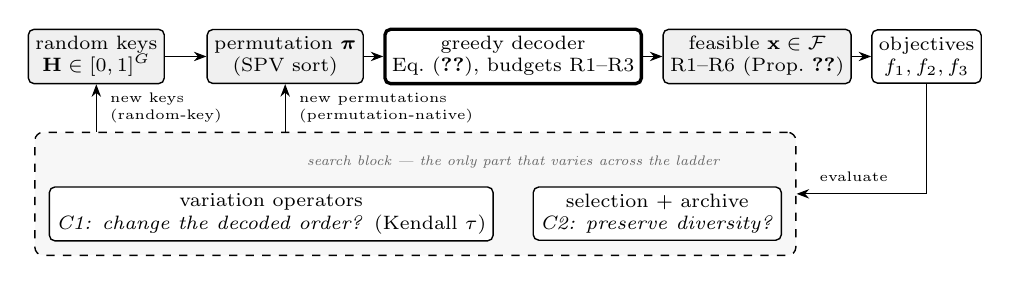
\begin{tikzpicture}[font=\scriptsize, >={Stealth[length=1.6mm]},
  box/.style={draw, rounded corners=2pt, align=center, inner sep=2.5pt,
              minimum height=15pt, line width=0.5pt},
  data/.style={box, fill=black!6},
  proc/.style={box, fill=white},
  node distance=10pt and 7pt]
% --- shared evaluation path (top row) ---
\node[data] (keys) {random keys\\$\mathbf{H}\in[0,1]^{G}$};
\node[data, right=15pt of keys] (perm) {permutation $\boldsymbol{\pi}$\\(SPV sort)};
\node[proc, very thick, right=of perm] (dec) {greedy decoder\\Eq.~(\ref{eq:greedy}), budgets R1--R3};
\node[data, right=of dec] (alloc) {feasible $\mathbf{x}\in\mathcal{F}$\\R1--R6 (Prop.~\ref{prop:feas})};
\node[proc, right=of alloc] (obj) {objectives\\$f_1,f_2,f_3$};
\draw[->] (keys) -- (perm);
\draw[->] (perm) -- (dec);
\draw[->] (dec) -- (alloc);
\draw[->] (alloc) -- (obj);
% --- search block (bottom row, swapped across the ladder) ---
\node[font=\tiny\itshape, text=black!60, below=22pt of dec.south] (blocklbl)
  {search block --- the only part that varies across the ladder};
\node[proc, below=3pt of blocklbl.south, anchor=north east, xshift=-7pt] (ops)
  {variation operators\\\textit{C1: change the decoded order?} (Kendall $\tau$)};
\node[proc, below=3pt of blocklbl.south, anchor=north west, xshift=7pt] (sel)
  {selection $+$ archive\\\textit{C2: preserve diversity?}};
\begin{scope}[on background layer]
\node[draw, dashed, rounded corners=3pt, fill=black!3, inner sep=5pt,
      fit=(blocklbl)(ops)(sel), line width=0.5pt] (block) {};
\end{scope}
\draw[->] (obj.south) |- node[above=1pt, font=\tiny, pos=0.78]{evaluate} (block.east);
\draw[->] (block.north -| keys.south) -- node[right=1.5pt, font=\tiny, align=left]
  {new keys\\(random-key)} (keys.south);
\draw[->] (block.north -| perm.south) -- node[right=1.5pt, font=\tiny, align=left]
  {new permutations\\(permutation-native)} (perm.south);
\end{tikzpicture}
\caption{The experimental design: a shared feasibility-preserving evaluation path (top; permutation-native methods enter it one step later) and the search block (bottom, shaded), the only component swapped across the method ladder. The diagnostic asks whether operators change the decoded order (C1) and selection preserves diversity (C2).}
\label{fig:pipeline}
\end{figure}

\subsection{Multi-objective Harris Hawks Optimization}
\label{sec:mohho}

Each hawk is a position $\mathbf{H}\in\mathbb{R}^{G}$ in the box $[0,1]^{G}$ (here $G=105$). At iteration $t$ the escape energy is
\begin{equation}
E = 2E_0\!\left(1 - \tfrac{t}{T}\right), \qquad E_0 \sim U(-1,1),
\label{eq:energy}
\end{equation}
which drives the choice among six movement operators selected by $|E|$ and uniform draws $q,r\in U(0,1)$: two exploration moves ($|E|\ge1$; relative to a random hawk or to the population centroid), a soft and a hard besiege toward the prey ($0.5\le|E|<1$ and $|E|<0.5$), and a L\'evy-dive variant of each besiege. The multi-objective adaptation draws the \emph{leader} (the ``rabbit'' of the HHO metaphor) from an external archive of non-dominated solutions with probability proportional to crowding distance, prunes the most crowded solution on overflow, and updates the archive after every move; the archive size is a tunable parameter (Section~\ref{sec:taguchi}). A hawk moves only if its trial dominates its current position (single-objective HHO's greedy replacement lifted to dominance; the published variants~\cite{jangir,cerci,kusoglu} do not specify this acceptance, so the naive configuration's failures characterize this choice, not those variants). For evaluation fairness, the L\'evy operators accept a single trial point per hawk per iteration (the canonical HHO evaluates two), so MOHHO, like every method, consumes exactly $N\times T$ evaluations.

\subsection{A feasibility-preserving decoder}
\label{sec:decoder}

The HHO operators act in the continuous space $\mathbb{R}^{G}$, but the problem is combinatorial with six hard constraints. We bridge the two with the SPV rule~\cite{bean,tasgetiren}---which turns a hawk $\mathbf{H}$ into a permutation $\boldsymbol{\pi}$ by sorting the group indices in ascending order of their key $h_g$---followed by a deterministic greedy assignment (Figure~\ref{fig:pipeline}) that walks the groups in SPV order and fixes the model's decision variable
\begin{equation}
x_g = \min\!\bigl(n_g,\; V_{\text{rem}},\; P^{\text{rem}}_{c(g)},\; K^{\text{rem}}_{j(g)}\bigr),
\label{eq:greedy}
\end{equation}
decrementing the residual budgets of R1--R3 after each step. No penalty term is introduced and no repair is performed: the hawks search directly on a feasible landscape. The greedy fill is budget-saturating (each visited group gets its maximal feasible amount), so the decoder's image is the saturating subset of $\mathcal{F}$ and all dominance claims are relative to it; an exact bi-objective $(f_1,f_3)$ mixed-integer linear program (MILP) (Section~\ref{sec:ablation}) confirms this subset loses nothing relevant.

\begin{proposition}[Feasibility by construction]
\label{prop:feas}
For any hawk $\mathbf{H}\in\mathbb{R}^{G}$, the allocation $\mathbf{x}$ returned by the SPV${}+{}$greedy decoder satisfies R1--R6.
\end{proposition}

\begin{proof}
Each step caps $x_g$ by every remaining budget and by $n_g$, so by induction every residual stays $\ge 0$ (R1--R3), while $0\le x_g\le n_g$ gives R4 and integrality gives R5; serving each group's $x_g$ most-senior petitions honors R6. \qed
\end{proof}

\subsection{Benchmarks and a representation-matched optimizer}
\label{sec:nsga}

The \emph{ladder} of methods shares the greedy decoder, objectives, hypervolume reference point, and $50\times500$ budget; the methods differ only in how they explore. Two operate on the continuous SPV random keys in $\mathbb{R}^{105}$:
\emph{(a)}~the MOHHO of Section~\ref{sec:mohho}; and
\emph{(b)}~\textbf{NSGA-II}~\cite{deb} with simulated binary crossover (SBX, $\eta_c=20$, $p_c=0.9$), polynomial mutation ($\eta_m=20$, $p_m=1/d$), binary tournament selection, and elitist $(\mu+\lambda)$ replacement.
A third, \emph{(c)}~\textbf{random restart}, draws all $25{,}000$ candidates uniformly at random, isolating the decoder's contribution.

The ablation (Section~\ref{sec:ablation}) reveals that the continuous random-key operators are a poor match for the induced permutation landscape. We therefore also evaluate \textbf{permutation-native} methods---spanning four distinct paradigms---that act directly on permutations of the 105 groups (decoded by the same greedy procedure): \emph{(d)}~\textbf{permutation-NSGA-II} (dominance-based) with order crossover (OX) and swap mutation; \emph{(e)}~\textbf{permutation-MOEA/D} (decomposition~\cite{zhangli}; Tchebycheff over 45 weight vectors, 10-nearest-neighborhood mating and replacement, archive 100, same OX${}+{}$swap); \emph{(f)}~\textbf{permutation-SPEA2}~\cite{spea2} (strength-Pareto, density-based truncation) under the same operators; and \emph{(g)}~\textbf{Discrete-MOHHO}, our representation-matched Harris Hawks optimizer: it keeps HHO's signature---the escape energy of Eq.~(\ref{eq:energy}) and a crowding-pruned external archive supplying the leader---but expresses every move on permutations (OX recombination with a random hawk or the leader, $|E|$-scaled swaps, occasional segment reversals). Discrete HHO variants exist for single-objective settings~\cite{gezici}; Discrete-MOHHO here is the matched swarm the mechanism check requires, not a novelty claim. Finally, we add \emph{(h)}~\textbf{rk-NSGA-II (biased uniform)}~\cite{goncalves}: the skeleton of \emph{(b)} with SBX and polynomial mutation replaced by BRKGA-style parameterized uniform crossover (elite-parent gene with probability $0.7$) and per-gene random-reset mutation---an order-changing random-key control used as a predictive test in Section~\ref{sec:ablation}; all methods run 30 seeds (1--30) under an identical budget.

\subsection{Evaluation protocol, indicators, and tuning}
\label{sec:protocol}

We assess each approximation front with the \emph{hypervolume} (\HV; larger is better) with respect to the reference point $(10;\,16;\,20{,}000)$, an upper bound on each objective; the \emph{inverted generational distance} (\IGD; smaller is better) to a reference front $Z$ formed by the non-dominated union of the MOHHO and NSGA-II combined fronts ($|Z|=126$; used only for that pairwise comparison---the ladder relies on \HV); the \emph{spacing} indicator; and the \emph{cardinality} of the non-dominated set (objectives min--max normalized before \IGD\ and spacing). Each algorithm runs for 30 independent seeds, and a \emph{combined front} is the non-dominated union of its 30 per-run fronts. Because every method runs on the common seed block 1--30, paired comparisons use the Wilcoxon signed-rank test (with the Mann--Whitney $U$~\cite{derrac} as an unpaired cross-check), and effect size is the Vargha--Delaney $A_{12}$~\cite{vargha}. The deterministic \textbf{FIFO} baseline orders groups by ascending priority date through the same decoder: $f_1=8.7891$, $f_2=13.0$ years, $f_3=1{,}940$ wasted visas.

%===============================================================================
\paragraph{Parameter tuning.}
\phantomsection\label{sec:taguchi}%
We replace empirical parameter choices by a Taguchi L9$(3^4)$ orthogonal-array design~\cite{alrafei,montgomery} over four factors at three levels: population $N\in\{30,50,70\}$, iteration budget $T\in\{100,300,500\}$, archive size $\in\{50,100,150\}$, and L\'evy exponent $\beta\in\{1.3,1.5,1.7\}$. The response is the larger-the-better signal-to-noise (S/N) ratio of the hypervolume, with each of the nine configurations replicated over 12 seeds disjoint from the evaluation seeds.

Averaging the S/N ratio per factor level gives an unambiguous ranking: population ($\Delta=0.318$~dB) and iteration budget ($\Delta=0.155$~dB) dominate, while $\beta$ ($0.108$~dB) and archive size ($0.046$~dB) lie within run-to-run noise. The additive model predicts the optimum $N{=}70$, $T{=}500$ at S/N $\approx109.77$~dB; a confirmation run gives $109.66$~dB ($\HV=304{,}391$), validating the model. The 30-run study adopts a deliberately conservative, compute-economical operating point: $N{=}50$, $T{=}500$, archive $100$, $\beta{=}1.5$. Its confirmation gives S/N $109.56$~dB---within $1.2\,\%$ in hypervolume of the L9 optimum, which differs only in $N{=}50$ vs.\ $70$. The full response table is in the repository.

%===============================================================================
\section{Results}
\label{sec:results}

\subsection{Combined Pareto front and domination of FIFO}
\label{sec:front}

Combining and re-filtering the 30 runs yields a front of 104 non-dominated solutions (Figure~\ref{fig:pareto2d}); the FIFO baseline is strictly dominated. The extreme solutions expose the trade-offs: radical equity ($f_1=8.9994$, $f_2=2.0$~yr, $f_3=0$), full utilization ($8.996$, $2.46$, $0$), and the minimum-$f_1$ solution that dominates FIFO---strictly better on waste ($f_3$ from 1{,}940 to 680 visas), tied on the maximal disparity ($f_2=13.0$), and negligibly better on the near-degenerate $f_1$ (8.7891 to 8.7884). The substantive case against FIFO is thus about waste and equity: 94 of the 104 front solutions reach $f_3=0$ (zero waste, which FIFO never attains), with disparities spanning from 13.0 years down to 2.0. (The MOHHO, Discrete-MOHHO, and permutation-NSGA-II combined fronts agree within $0.3\,\%$ in hypervolume.) Convergence is fast and stable: the mean hypervolume reaches 99\,\% of its final value by iteration~135, and over the 30 runs the \HV\ distribution is narrow (mean $302{,}756$, coefficient of variation [CV] $2.36\,\%$).

\begin{figure}[t]
\centering

\includegraphics[width=0.50\textwidth]{pareto_f1f2.pdf}
\caption{The $f_1$--$f_2$ projection of the 104-solution combined Pareto front, colored by the third objective $f_3$ (wasted visas). The FIFO baseline (star) is strictly dominated.}
\label{fig:pareto2d}
\end{figure}

\subsection{Decoder, representation, and search: a controlled ladder}
\label{sec:ablation}

The ladder results (Table~\ref{tab:ladder}, Figure~\ref{fig:ladder}) attribute performance to its true source; the permutation-native methods inherit the Taguchi-tuned $N$ and $T$ and are not separately tuned, so any edge is not a tuning artifact. Under this budget MOHHO beats the real-coded NSGA-II by $3.2\,\%$ in mean hypervolume (paired two-sided Wilcoxon $p=4.4\times10^{-6}$, $A_{12}=0.85$) and shows lower spacing (NSGA-II edges it on \IGD\ to the combined reference front).

\paragraph{Blind sampling beats near-identity search---but not a competent swarm.}
\emph{Random restart}---blind sampling with no search---already reaches a mean \HV\ of $310{,}214$: $5.7\,\%$ above the real-coded NSGA-II and $2.5\,\%$ above the classic real-coded MOHHO (the naive swarm wins on only $10/30$ paired seeds). Giving NSGA-II the same external archive barely helps ($293{,}666$ vs.\ $293{,}367$), so the deficit is no archiving artifact.

Nor is blind sampling's strength order-level greediness: a GRASP-style semi-greedy control~\cite{feo} ($\alpha\sim U(0,1)$, same budget) lands $3.8\,\%$ below uniform constructions ($298{,}531$, $p=1.9\times10^{-9}$)---the decoder's heuristic bias~\cite{raidl} helps every construction. Nor is it tuning: NSGA-II's own L9 (best confirmed on the 30-seed block: $\eta_c{=}2$, $p_m{=}5/d$) climbs to $308{,}082$, a statistical tie with blind sampling ($p=0.25$), still $3.2\,\%$ below the permutation tier; a Pareto local search (single swaps are near-identity, so the diagnostic predicts failure) lands $2.0\,\%$ below blind sampling ($p=3.4\times10^{-4}$). With the registered sweep below, five controls tell one story: nothing we tested short of order renewal beats blind sampling here. To show that what fails is degenerate search rather than real-coded search as such, we built a \emph{competent} real-coded MO-HHO: HHO movement with elitist non-dominated-sorting selection and polynomial mutation in place of the dominance-gated acceptance. It is sound where the naive swarm collapses (ZDT2: $0.99$ vs.\ $0.20$ of the true front's hypervolume), and on the visa it beats random restart ($316{,}347$ vs.\ $310{,}214$, $+2.0\,\%$, paired Wilcoxon $p=5.7\times10^{-4}$, 30 seeds).

\paragraph{Why near-identity operators fail.}
We measured why the real-coded NSGA-II falls below blind sampling. On the SPV random keys, SBX and polynomial mutation are near-identity on the decoded permutation: over $3{,}000$ trials the Kendall rank correlation between a parent's SPV order and its child's is $\tau=0.99$ (and stays in $[0.987,0.992]$ along the search trajectory). Sweeping the crossover distribution index $\eta_c\in\{2,\dots,100\}$ confirms this is no tuning artifact: even the most disruptive setting ($\eta_c{=}2$, $\tau{=}0.92$) leaves the GA's mean \HV\ at $305{,}293$, below blind random restart---the GA perturbs the keys so little that the induced permutation barely changes, leaving it almost frozen in combinatorial space. HHO's position updates, by contrast, propose large permutation jumps ($\tau\approx0$) that the dominance-gated acceptance rarely admits (only ${\sim}0.6\,\%$ of hawks move per iteration), but the archive keeps the rejected proposals---hence MOHHO $>$ NSGA-II within the random-key tier. The real-coded MOHHO is thus a deliberately standard, weak baseline (its ZDT2 collapse persists under every acceptance rule and repair we tried): the thesis rests on degenerate search losing even to blind sampling, not on swarm strength.

\paragraph{Matching the operators to the representation.}
The clean fix is to act directly on permutations. Doing so lifts four distinct paradigms above blind sampling: permutation-NSGA-II (dominance/GA) reaches $318{,}151$, permutation-SPEA2 (strength-Pareto) $317{,}135$, Discrete-MOHHO (swarm) $316{,}792$, and permutation-MOEA/D (decomposition) $314{,}846$---and the competent random-key swarm joins them ($316{,}347$), so the encoding is not the divider. The four cluster within about $1\,\%$ of one another (permutation-SPEA2 vs.\ permutation-NSGA-II: $p=0.47$, a statistical tie), yet all sit $1.5$--$2.6\,\%$ above blind random restart. Discrete-MOHHO improves on classic MOHHO by $+4.6\,\%$ (paired Wilcoxon $p=9.3\times10^{-10}$, better on all $30/30$ seeds); the most stable methods are matched ones (permutation-NSGA-II CV $0.58\,\%$, Discrete-MOHHO $0.71\,\%$, vs.\ classic MOHHO $2.36\,\%$), permutation-NSGA-II leading Discrete-MOHHO by $+0.43\,\%$ in mean \HV. Made representation-matched, the swarm reaches the top tier with low variance---a mechanism check rather than a champion claim (replacing its energy schedule by run-average constants shifts \HV\ by $+0.01\,\%$, $p=0.87$: the metaphor's scheduling is not a measurable driver here~\cite{aranha,sorensen}).

\paragraph{The two conditions, graded by a predictive test.}
The ladder suggests a two-condition rule for this landscape: a method beats blind sampling only if its operator changes the decoded order ($\tau$ far from $1$) and its selection preserves population diversity (non-dominated sorting, strength-Pareto, decomposition, or a crowded archive---not dominance-gated acceptance). NSGA-II fails the first; the naive MOHHO fails the second; the competent MO-HHO and all four permutation-native methods satisfy both and beat random restart. We then tested the rule predictively on a method not used to formulate it: the rk-NSGA-II (biased uniform) of Section~\ref{sec:nsga}, whose BRKGA-style crossover changes the decoded order ($\tau=0.63\pm0.07$) under unchanged diversity-preserving selection. Read as a binary conjunction, the rule predicts a win over blind sampling. The prediction fails: the method's mean \HV\ of $309{,}970$ is a statistical tie with random restart ($310{,}214$; paired Wilcoxon $p=0.79$, $A_{12}=0.47$); a canonical BRKGA ($20\,\%$ elites, $15\,\%$ mutants, same crossover) lands at the same level ($309{,}928$). The test refines the rule: both conditions are necessary but not sufficient. Holding the diversity-preserving selection fixed while varying only the operator gives an ordered four-point sequence---$\tau{=}0.99\!\to\!293{,}367$; $\tau{=}0.92\!\to\!305{,}293$; $\tau{=}0.63\!\to\!309{,}970$; $\tau{\approx}0\!\to\!315{,}730$ (Section~\ref{sec:twoconditions}). A second registered sweep (predictions committed before running: the biased-uniform crossover's inheritance probability $\rho_e$, eleven levels spanning $\tau\in[0.42,1.0]$, fixed selection, all five structures, 30 seeds per level) shows this is a family contrast, not a dose--response: within the family, hypervolume is nearly flat in $\tau$ on every structure (Spearman $-0.07$ to $0.48$, n.s.), while \IGD$^{+}$ against the pooled sweep front does degrade as $\tau\to1$ on three of the five ($\rho\ge0.80$). So $\tau$ is a flag, not a dial; only a coverage metric sees the residual dose effect.

\paragraph{An empirical regularity.}
That encoding--operator mismatch can hurt search has been known since random keys were introduced~\cite{bean}, with the locality of decoder-based encodings formalized by Rothlauf~\cite{rothlauf} and measured by Raidl and Gottlieb~\cite{raidl}; our contribution is the controlled, multi-method, causally graded demonstration on a real constrained multi-objective problem---including that both real-coded searches fall below blind sampling. Within a matched representation both the operator set and the selection architecture are second-order (a $3\times3$ operator${}\times{}$architecture factorial attributes only $5.5\,\%$ and $13.4\,\%$ of the hypervolume variance to them, against $78\,\%$ seed noise). A paired Friedman test with a Nemenyi post-hoc~\cite{demsar} across all nine ladder methods rejects equal performance decisively ($\chi^2=133.8$, $p\approx4.6\times10^{-25}$, critical difference $2.19$) and ranks them as the two-condition account predicts (permutation-NSGA-II $2.97$ best, real-coded NSGA-II $8.77$ worst; rk-NSGA-II $4.57$, within the critical difference of random restart $6.47$); all twelve headline pairwise claims survive a Holm correction, and re-scoring every per-run front under \IGD$^{+}$ and additive $\epsilon$ keeps four of the five both-condition methods in the top four ranks (permutation-MOEA/D is the one displacement; rank correlations $0.82$/$0.85$ with \HV)---an empirical regularity for this problem, not a general law.

\begin{table}[t]
\centering
\caption{The method ladder: 30 runs each, identical greedy decoder and $25{,}000$-evaluation budget. Top block: random-key encoding; bottom block: permutation-native. Best per column in bold (rk-NSGA-II's best combined front reflects its bimodal between-run dispersion; per-run it only ties blind sampling); ``perm-'' abbreviates ``permutation-''.}
\label{tab:ladder}
\footnotesize
\begin{tabular}{llccrr}
\toprule
\textbf{Method} & \textbf{Paradigm} & \textbf{Mean \HV\ $\pm\,\sigma$} & \textbf{CV} & \textbf{Comb.\ \HV} & \textbf{\#\,sols}\\
\midrule
NSGA-II            & GA       & $293{,}367 \pm 6{,}996$ & 2.38\,\% & 316{,}060 & 92\\
MOHHO              & swarm    & $302{,}756 \pm 7{,}138$ & 2.36\,\% & 320{,}984 & 104\\
rk-NSGA-II (biased unif.) & GA & $309{,}970 \pm 9{,}790$ & 3.16\,\% & \textbf{325{,}465} & 157\\
Random restart     & ---      & $310{,}214 \pm 2{,}735$ & 0.88\,\% & 317{,}673 & 65\\
Competent MO-HHO   & swarm    & $316{,}347 \pm 6{,}683$ & 2.11\,\% & 321{,}800 & \textbf{207}\\
\midrule
perm-MOEA/D                 & decomp.\ & $314{,}846 \pm 5{,}384$  & 1.71\,\% & 320{,}969 & 90\\
Discrete-MOHHO              & swarm    & $316{,}792 \pm 2{,}258$  & 0.71\,\% & 321{,}408 & 137\\
perm-SPEA2                  & str.-Pareto & $317{,}135 \pm 3{,}814$ & 1.20\,\% & 322{,}037 & 179\\
perm-NSGA-II                & GA       & $\mathbf{318{,}151 \pm 1{,}855}$ & \textbf{0.58\,\%} & 321{,}935 & 148\\
\bottomrule
\end{tabular}
\end{table}

\begin{figure}[t]
\centering

\includegraphics[width=0.71\textwidth]{ladder.pdf}
\caption{The nine-method ladder: per-run hypervolume (30 runs each, identical decoder and budget). The divider is non-degenerate search, not the encoding: the BRKGA-style rk-NSGA-II only ties blind random restart; the competent MO-HHO joins the top tier.}
\label{fig:ladder}
\end{figure}

\paragraph{Robustness to a search-space-collapse confound.}
Does the decoder's budget saturation make the optimizer necessarily second-order? Three checks bound this confound. \emph{Structure}: $50{,}000$ random permutations decode to $39{,}401$ distinct objective points (degeneration ratio $1.27$), and a principal-component analysis places about $99\,\%$ of the front's variance in two components (the first alone captures $0.81$--$0.91$)---a near-mono-objective instance with one wide axis ($f_2$). \emph{Decoder}: re-running the full ladder on two \emph{non-saturating} decoders (fractional-intensity and stochastic-skip, both feasible by construction) keeps the permutation tier above the random-key tier under all three decoders (paired Wilcoxon $p<10^{-3}$); the margin shrinks from $6.9\,\%$ (greedy) to $4.3\,\%$ (stochastic-skip) and $1.4\,\%$ (fractional-intensity), so saturation amplifies---it does not create---the effect, and an exact $(f_1,f_3)$ MILP front ($f_2$---a maximum over differences of ratios of decision variables---is outside MILP form and evaluated a posteriori) exposes no practically meaningful non-saturating solution the greedy front misses. \emph{Metric}: the per-run tier ranking is reference-point-robust (four of five reference points), though on combined fronts the strict tier softens under reference-free metrics. The confound thus bounds rather than overturns the claim: the effect is real and robust, modest on this saturation-amplified, $f_2$-dominated instance, with the general regularity resting on the additional structures below.

\subsection{Isolating the two conditions: a controlled $2\times2$}
\label{sec:twoconditions}
The ladder establishes the two conditions by observation; we now isolate each condition with a controlled $2\times2$ on a single real-coded random-key skeleton---same greedy decoder, instance, $25{,}000$-evaluation budget, and 30 seeds---varying only the \emph{operator} (order-changing HHO moves with mutation, $\tau\!\approx\!0$, vs.\ near-identity SBX, $\tau\!=\!0.99$) and the \emph{selection} (diversity-preserving non-dominated sorting (NDS) vs.\ dominance-gated acceptance). Figure~\ref{fig:mech2x2} shows that only the cell satisfying both conditions beats blind random restart ($315{,}730$ vs.\ $310{,}214$~\HV, $+1.78\,\%$, paired Wilcoxon $p=1.4\times10^{-3}$, $A_{12}=0.79$); either single-condition cell falls below blind sampling, losing by $1.4$--$2.0\,\%$. Gated acceptance freezes the population (only $0.9\,\%$ of individuals move per iteration), and near-identity SBX leaves the decoded order almost unchanged even when the population does move. Crucially, the two conditions are synergistic, not additive: a two-factor analysis of variance finds a significant operator$\times$selection interaction ($\eta^2=0.098$, $F=16.7$, $p=8.0\times10^{-5}$; a permutation test agrees, $p=2.0\times10^{-4}$), alongside main effects of $\eta^2=0.076$ (operator) and $\eta^2=0.145$ (selection); the interaction is what separates beating blind sampling from losing to it.

\begin{figure}[t]
\centering

\includegraphics[width=0.64\textwidth]{mechanism_2x2_annot.pdf}
\caption{The controlled $2\times2$: each cell sits at its operator's order-preservation $\tau$ and its realized population movement, annotated with mean hypervolume, gap to blind random restart (\HV\ $310{,}214$), and $A_{12}$. Only the cell meeting both conditions (circle) beats blind sampling.}
\label{fig:mech2x2}
\end{figure}

\subsection{Generalization}
\label{sec:secondproblem}

\paragraph{Perturbed-demand instances.}
Five further instances perturbing every group's demand by an independent uniform $\pm 20\,\%$ (fixed seeds, recomputed caps) reproduce the pattern: FIFO is dominated on all five, MOHHO's mean \HV\ exceeds NSGA-II's (one-sided Mann--Whitney, directionally consistent on five of five, two individually significant; descriptive robustness, not confirmatory evidence), and random restart matches or exceeds MOHHO ($101$--$103\,\%$ of its \HV).

\paragraph{Structurally distinct problems.}
We replicate the six-method core of the ladder on three classic structures that share only the SPV${}+{}$greedy/permutation methodology: a 0/1 multidimensional knapsack (MOMKP, a \emph{selection} landscape), a tri-objective traveling-salesman problem (mo-TSP, \emph{sequencing}), and a tri-objective permutation flow-shop (mo-PFSP, \emph{scheduling}); same budget, 30 common seeds, paired Friedman${}+{}$Nemenyi (Figure~\ref{fig:structranks}). One result is robust across all four structures: among the six core ladder methods the best optimizer is always a permutation-native method, and neither blind random restart nor any naive real-coded method ever wins (all four omnibus tests reject equality, $\chi^2=112$--$150$, $p<10^{-21}$). Added as a seventh method on all four structures, the competent random-key MO-HHO of Section~\ref{sec:ablation} wins outright on the knapsack (mean rank 1.13 of seven) and ranks 2nd, 2nd, and 5th on the visa, flow-shop, and TSP. So the regularity is sharper than ``permutation beats random-key'': what wins on every structure is a method satisfying both conditions. What does not generalize is the dramatic ``GA below random sampling'': it holds on the selection landscapes (visa, knapsack, where the real-coded NSGA-II is worst) but reverses on the sequencing landscapes (TSP, flow-shop, where it is competitive and random restart is worst instead). The mechanism: operator order-preservation is problem-independent ($\tau\approx0.99$), but its consequence is landscape-dependent---near-identity SBX freezes search on selection landscapes yet acts as useful local search on sequencing ones. Tuning sharpens this: NSGA-II's own L9 on the knapsack lifts it $46\,\%$ above blind sampling ($p=1.9\times10^{-9}$; again via $p_m{=}5/d$)---the knapsack collapse is a default-configuration artifact; the configuration-robust collapse is the visa's alone. A fifteen-point capacity sweep rules out a single headroom scalar (it moves opposite to the hypothesis; Spearman $\rho=-0.78$, $p=0.001$, descriptive).

\begin{figure}[t]
\centering

\includegraphics[width=0.86\textwidth]{struct_ranks.pdf}
\caption{Mean Friedman rank (lower is better; 30 paired seeds) of the six core ladder methods on the four structures. Stars mark the best method per structure---always a permutation-native one (solid lines) among the six core methods shown; the real-coded NSGA-II (dashed) falls below blind random restart only on the budget-saturating landscapes (left).}
\label{fig:structranks}
\end{figure}

\paragraph{A registered prospective test.}
As a final check we registered the diagnostic's four predictions for a fifth, unseen problem before running any optimizer on it (the registration commit precedes the results in the repository): a tri-objective set-covering problem (mo-SCP; 150 elements, 120 sets, three cost vectors; the SPV decoder adds a set iff it covers a new element), labeled a selection landscape by its subset structure. The two predictions following from the two conditions alone held: permutation-NSGA-II and the competent swarm beat blind sampling decisively ($p=9.3\times10^{-10}$, $A_{12}=1.0$ for both). The two tied to the landscape label failed, informatively: the real-coded NSGA-II finishes $10\,\%$ above blind sampling and the biased-uniform rk-NSGA-II is the single best method ($+60\,\%$, above even permutation-NSGA-II). Mechanistically, mo-SCP saturates no shared budget---every decode is a feasible cover---so it behaves like a sequencing landscape (local search useful, blind sampling weak). The test confirms the two-condition core and falsifies the surface label as a classifier (the confirmed half carried less falsification risk on this blind-sampling-weak landscape). The operative determinant remains the registered open question; we hypothesize decoder budget saturation, consistent with the headroom anti-correlation. A first operationalization---the saturation share $s$ over random decodes, seconds to compute---retrodicts the default-collapse split ($s\approx1$ visa/knapsack, $0$ elsewhere) but awaits a registered test on unseen problems.

%===============================================================================
\section{Discussion}
\label{sec:discussion}

\paragraph{The trade-off is structural.}
Two countries hold roughly three-quarters of demand with 10--13-year waits; the $7\,\%$ ceiling forbids fully serving them, so reducing disparity ($f_2$) leaves unserved load ($f_1\!\uparrow$) and equitable spreading idles saturated categories ($f_3\!\uparrow$)---genuine three-way conflict, with the three extreme solutions mutually non-dominated. We keep $f_1$ distinct (its range is an order of magnitude narrower than $f_2$'s) because the minimum-$f_1$ policy is the one dominating FIFO.

\paragraph{A diagnostic protocol, and policy.}
The ladder distills into a cheap a priori protocol: (1)~draw ${\sim}3{,}000$ parent--child pairs through the candidate operators and measure the Kendall $\tau$ of the decoded orders; (2)~check that selection preserves diversity (NDS, strength-Pareto, decomposition, or a crowded archive---not gated acceptance); (3)~measure how strong blind sampling is on the decoded space (run it; it is the cheapest method) rather than classifying by surface structure---our registered prospective test (Section~\ref{sec:secondproblem}) shows the label can mispredict. On the budget-saturating problems, failing either check predicted default-configuration performance at or below blind sampling (the one nominal exception---the naive knapsack swarm---lies within the critical difference); on the visa, where blind sampling sits within $2.6\,\%$ of the best tier, no random-key GA configuration beats it. The protocol complements general fitness-landscape analysis~\cite{malan}: it measures the operator--decoder interaction rather than the landscape alone. Invest in the decoder and representation before the search heuristic; for a dependable single run, permutation-NSGA-II is strongest here. For policy, the front is a quantified menu under the assumed model: cutting disparity from 13.0 to 2.0 years costs only $\sim$$2.4\,\%$ in $f_1$ relative to FIFO---consistent with per-country-cap reform proposals~\cite{crs,fwd}; each solution maps to an auditable per-country reallocation.

\paragraph{Limitations.}
The model covers a single fiscal year, uses 21 representative countries, aggregates each group to a single priority date, and assumes every assigned visa is used. The country-level totals are anchored to published aggregates~\cite{cato,uscis,dos}, but the per-(country, category) split and priority dates are a plausible synthetic disaggregation (only India, China, the Philippines, and Mexico have category-level demand grounded in published data). These affect external validity, not the internal comparison: the ladder methods share identical data, decoder, and budget. \emph{Ethically}, $f_2$ encodes one contestable notion of fairness and treats nationalities as allocation buckets; we therefore present the front as auditable decision support, never an autonomous decision-maker, and the per-country figures illustrate method behavior rather than recommend real allocations. A post-hoc audit with alternative country-wait metrics (wait standard deviation $3.14\to0.75$, Gini $0.79\to0.17$, Jain $0.80\to0.94$) supports the same equity reading.

%===============================================================================
\section{Conclusions}
\label{sec:conclusions}

We formulated a calibrated instance of the annual allocation of U.S.\ employment-based visas as a three-objective integer program with six hard constraints and searched the decoder-reachable trade-off space through a feasibility-preserving SPV${}+{}$greedy decoder---no penalties, no repair---under a Taguchi-fixed operating point shared by every method. Across 30 independent runs the recovered Pareto front dominates the FIFO incumbent, chiefly by reducing waste, with 94 zero-waste solutions. Our central result comes from a controlled nine-method ladder: blind random sampling beats a standard real-coded NSGA-II and the naive real-coded MOHHO swarm, but a competent real-coded swarm beats blind sampling by $2.0\,\%$---so what fails is degenerate search, not real-coded search as such. The lesson is a two-condition screening diagnostic, scoped and graded: a method that does not change the decoded order or does not preserve population diversity falls to or below blind sampling (within the critical difference) at the default configuration on the budget-saturating problems---and under every configuration we tested on the visa. The conditions are necessary but not sufficient (the BRKGA-style predictive test only ties blind sampling), and graded as a family contrast rather than a dose--response (the registered sweep): only the right kind of order renewal reaches the top tier, where four permutation-native paradigms and a competent random-key swarm cluster within about $1\,\%$---the divider is non-degenerate search, not the encoding.

The findings are directionally consistent across five perturbed-demand instances, and the cross-structure study sharpens what generalizes: the best ladder method on every structure satisfies both conditions, whereas the collapse of a mismatched GA below blind sampling is landscape- and configuration-specific---configuration-robust only on the visa. A registered prospective test on a fifth problem (set covering) confirms the core and falsifies the surface landscape label. Beyond the numbers, the method yields an auditable menu of feasible trade-offs as decision support, not a policy prescription. Future work includes a multi-period formulation, the full country roster, and a registered test of the budget-saturation hypothesis as the landscape determinant.

%===============================================================================
\subsubsection*{Data and Code Availability.}
The data, optimizer, Taguchi design, and all scripts are available at \url{https://github.com/jrebull/MIAAD_Harrisv2} (tag \texttt{micai-submission-v2}); fixed seeds (diagnostic suite: 1; comparisons: 1--30) regenerate every reported number deterministically.
% >>> REVIEW: remove the URL above for double-blind submission.

\subsubsection*{Acknowledgments.}
% >>> REVIEW: omit this block for double-blind submission.
The authors thank the Universidad Aut\'onoma de Ciudad Ju\'arez for institutional support.

%===============================================================================
\begin{thebibliography}{99}

\bibitem{alrafei}
Al Rafei, T., Yousfi Steiner, N., Chrenko, D.: Genetic algorithm and Taguchi method: an approach for better Li-ion cell model parameter identification. Batteries \textbf{9}(2), 72 (2023). \doi{10.3390/batteries9020072}

\bibitem{aranha}
Aranha, C., Camacho Villal\'on, C.L., Campelo, F., Dorigo, M., Ruiz, R., Sevaux, M., et al.: Metaphor-based metaheuristics, a call for action: the elephant in the room. Swarm Intelligence \textbf{16}(1), 1--6 (2022). \doi{10.1007/s11721-021-00202-9}

\bibitem{bansak}
Bansak, K., Ferwerda, J., Hainmueller, J., Dillon, A., Hangartner, D., Lawrence, D., et al.: Improving refugee integration through data-driven algorithmic assignment. Science \textbf{359}(6373), 325--329 (2018). \doi{10.1126/science.aao4408}

\bibitem{bean}
Bean, J.C.: Genetic algorithms and random keys for sequencing and optimization. ORSA Journal on Computing \textbf{6}(2), 154--160 (1994). \doi{10.1287/ijoc.6.2.154}

\bibitem{cato}
Bier, D.J.: 1.8 million in employment-based green card backlog. Cato Institute, Washington, DC (2023), \url{https://www.cato.org/blog/18-million-employment-based-green-card-backlog}

\bibitem{chaves}
Chaves, A.A., Resende, M.G.C., Schuetz, M.J.A., Brubaker, J.K., Katzgraber, H.G., de Arruda, E.F., et al.: A random-key optimizer for combinatorial optimization. Journal of Heuristics \textbf{31}(4), 32 (2025). \doi{10.1007/s10732-025-09568-z}

\bibitem{choo}
Choo, Y.H., Cai, Z., Le, V., Johnstone, M., Creighton, D., Lim, C.P.: Enhancing the Harris' Hawk optimiser for single- and multi-objective optimisation. Soft Computing \textbf{27}(22), 16675--16715 (2023). \doi{10.1007/s00500-023-08952-w}

\bibitem{coello}
Coello Coello, C.A., Lamont, G.B., Van Veldhuizen, D.A.: Evolutionary Algorithms for Solving Multi-Objective Problems, 2nd edn. Springer, New York (2007). \doi{10.1007/978-0-387-36797-2}

\bibitem{crs}
Congressional Research Service: U.S. employment-based immigration policy. Report R47164 (2023), \url{https://www.congress.gov/crs-product/R47164}

\bibitem{deb}
Deb, K., Pratap, A., Agarwal, S., Meyarivan, T.: A fast and elitist multiobjective genetic algorithm: NSGA-II. IEEE Transactions on Evolutionary Computation \textbf{6}(2), 182--197 (2002). \doi{10.1109/4235.996017}

\bibitem{demsar}
Demšar, J.: Statistical comparisons of classifiers over multiple data sets. Journal of Machine Learning Research \textbf{7}, 1--30 (2006), \url{https://jmlr.org/papers/v7/demsar06a.html}

\bibitem{derrac}
Derrac, J., García, S., Molina, D., Herrera, F.: A practical tutorial on the use of nonparametric statistical tests as a methodology for comparing evolutionary and swarm intelligence algorithms. Swarm and Evolutionary Computation \textbf{1}(1), 3--18 (2011). \doi{10.1016/j.swevo.2011.02.002}

\bibitem{feo}
Feo, T.A., Resende, M.G.C.: Greedy randomized adaptive search procedures. Journal of Global Optimization \textbf{6}(2), 109--133 (1995). \doi{10.1007/BF01096763}

\bibitem{fwd}
FWD.us: Per-country cap reform: priority bill spotlight (2024), \url{https://www.fwd.us/news/per-country-cap-reform-priority-bill-spotlight/}

\bibitem{garey}
Garey, M.R., Johnson, D.S.: Computers and Intractability: A Guide to the Theory of NP-Completeness. W.H. Freeman, San Francisco (1979)

\bibitem{gezici}
Gezici, H., Livatyali, H.: An improved Harris Hawks Optimization algorithm for continuous and discrete optimization problems. Engineering Applications of Artificial Intelligence \textbf{113}, 104952 (2022). \doi{10.1016/j.engappai.2022.104952}

\bibitem{goncalves}
Gon\c{c}alves, J.F., Resende, M.G.C.: Biased random-key genetic algorithms for combinatorial optimization. Journal of Heuristics \textbf{17}(5), 487--525 (2011). \doi{10.1007/s10732-010-9143-1}

\bibitem{heidari}
Heidari, A.A., Mirjalili, S., Faris, H., Aljarah, I., Mafarja, M., Chen, H.: Harris hawks optimization: algorithm and applications. Future Generation Computer Systems \textbf{97}, 849--872 (2019). \doi{10.1016/j.future.2019.02.028}

\bibitem{jangir}
Jangir, P., Heidari, A.A., Chen, H.: Elitist non-dominated sorting Harris hawks optimization: framework and developments for multi-objective problems. Expert Systems with Applications \textbf{186}, 115747 (2021). \doi{10.1016/j.eswa.2021.115747}

\bibitem{londe}
Londe, M.A., Pessoa, L.S., Andrade, C.E., Resende, M.G.C.: Biased random-key genetic algorithms: a review. European Journal of Operational Research \textbf{321}(1), 1--22 (2025). \doi{10.1016/j.ejor.2024.03.030}

\bibitem{malan}
Malan, K.M., Engelbrecht, A.P.: A survey of techniques for characterising fitness landscapes and some possible ways forward. Information Sciences \textbf{241}, 148--163 (2013). \doi{10.1016/j.ins.2013.04.015}

\bibitem{montgomery}
Montgomery, D.C.: Design and Analysis of Experiments, 9th edn. Wiley, Hoboken (2017)

\bibitem{rahimi}
Rahimi, I., Gandomi, A.H., Chen, F., Mezura-Montes, E.: A review on constraint handling techniques for population-based algorithms: from single-objective to multi-objective optimization. Archives of Computational Methods in Engineering \textbf{30}(3), 2181--2209 (2023). \doi{10.1007/s11831-022-09859-9}

\bibitem{raidl}
Raidl, G.R., Gottlieb, J.: Empirical analysis of locality, heritability and heuristic bias in evolutionary algorithms: a case study for the multidimensional knapsack problem. Evolutionary Computation \textbf{13}(4), 441--475 (2005). \doi{10.1162/106365605774666886}

\bibitem{rothlauf}
Rothlauf, F.: Representations for Genetic and Evolutionary Algorithms, 2nd edn. Springer, Berlin, Heidelberg (2006). \doi{10.1007/3-540-32444-5}

\bibitem{sorensen}
S\"orensen, K.: Metaheuristics---the metaphor exposed. International Transactions in Operational Research \textbf{22}(1), 3--18 (2015). \doi{10.1111/itor.12001}

\bibitem{tasgetiren}
Tasgetiren, M.F., Liang, Y.-C., Sevkli, M., Gencyilmaz, G.: A particle swarm optimization algorithm for makespan and total flowtime minimization in the permutation flowshop sequencing problem. European Journal of Operational Research \textbf{177}(3), 1930--1947 (2007). \doi{10.1016/j.ejor.2005.12.024}

\bibitem{uscis}
U.S. Citizenship and Immigration Services: Fiscal year 2023 employment-based adjustment of status FAQs (2023), \url{https://www.uscis.gov/green-card/green-card-processes-and-procedures/fiscal-year-2023-employment-based-adjustment-of-status-faqs}

\bibitem{dos}
U.S. Department of State: Visa bulletin for February 2026 (2026), \url{https://travel.state.gov/content/travel/en/legal/visa-law0/visa-bulletin/2026/visa-bulletin-for-february-2026.html}

\bibitem{vargha}
Vargha, A., Delaney, H.D.: A critique and improvement of the CL common language effect size statistics of McGraw and Wong. Journal of Educational and Behavioral Statistics \textbf{25}(2), 101--132 (2000). \doi{10.3102/10769986025002101}

\bibitem{cerci}
Wang, M., Wang, J.-S., Song, H.-M., Zhang, M., Zhang, X.-Y., Zheng, Y., et al.: Hybrid multi-objective Harris Hawk optimization algorithm based on elite non-dominated sorting and grid index mechanism. Advances in Engineering Software \textbf{172}, 103218 (2022). \doi{10.1016/j.advengsoft.2022.103218}

\bibitem{kusoglu}
Yüzgeç, U., Kuşoğlu, M.: Multi-objective Harris Hawks optimizer for multiobjective optimization problems. BSEU Journal of Engineering Research and Technology \textbf{1}(1), 31--41 (2020), \url{https://bseujert.bilecik.edu.tr/index.php/bseujert/article/view/14}

\bibitem{zhangli}
Zhang, Q., Li, H.: MOEA/D: a multiobjective evolutionary algorithm based on decomposition. IEEE Transactions on Evolutionary Computation \textbf{11}(6), 712--731 (2007). \doi{10.1109/TEVC.2007.892759}

\bibitem{zhang}
Zhang, W., Xiao, G., Gen, M., Geng, H., Wang, X., Deng, M., et al.: Enhancing multi-objective evolutionary algorithms with machine learning for scheduling problems: recent advances and survey. Frontiers in Industrial Engineering \textbf{2}, 1337174 (2024). \doi{10.3389/fieng.2024.1337174}

\bibitem{spea2}
Zitzler, E., Laumanns, M., Thiele, L.: SPEA2: improving the strength Pareto evolutionary algorithm. TIK-Report 103, Computer Engineering and Networks Laboratory (TIK), ETH Zurich (2001). \doi{10.3929/ethz-a-004284029}

\bibitem{zitzler}
Zitzler, E., Thiele, L.: Multiobjective evolutionary algorithms: a comparative case study and the strength Pareto approach. IEEE Transactions on Evolutionary Computation \textbf{3}(4), 257--271 (1999). \doi{10.1109/4235.797969}

\end{thebibliography}

\end{document}
